\documentclass[12pt,a4paper]{article}
\usepackage[brazil]{babel}  %Suporte a PT-BR
%\usepackage[utf8]{inputenc} %Não necessário com XeLaTeX, suporta acentos
\usepackage{graphicx} %Importar imagens
\graphicspath{{./img/}}
\usepackage{amsmath} %Equações
\usepackage{float} %Inserir imagens in situ
\usepackage{listingsutf8} %Código com acentos
\usepackage{styles/c++} %Estilo, fica na pasta
\usepackage[backend=biber]{biblatex} %Suporte à Bibliografia
\addbibresource{references.bib}

\title{Relatório da Prática 7}
\author{Vítor Barbosa}
\date{\today}

\begin{document}
\maketitle

\section{Introdução}
Nesta prática há duas tarefas. A Tarefa 1 consiste em implementar um exemplo de sincronização de threads com mutex e semáforo e elucidar seu funcionamento.
A Tarefa 2 consiste em aplicar esses conceitos de sincronização a uma aplicação com GUI, usando threads ou runnables, além de algum mecanismo de exclusão mútua.

\section{Tarefa 1}
O programa desta tarefa implementa um exemplo de treino de Fórmula 1 com threads. São criadas 10 threads, que correspondem a 10 carros. Cada carro é atribuído a uma equipe aleatória (de 7 \emph{scuderias} possíveis) no momento de sua criação. Podem haver até 5 carros na pista, mas apenas 1 de cada equipe.

O código do programa está contido no arquivo \emph{formula1.cpp}
\subsubsection*{formula1.cpp}
\lstinputlisting[language=C++,style=c++]{../Aula7_mutex_console/formula1.cpp}

\subsubsection*{O que ocorre no Mutex}

Há um array de 7 mutexes, um por equipe. Quando um carro entra na pista, isto é, sua thread é executada pelo método \emph{beginthreadex}, ele tenta adquirir o mutex "M" de sua equipe. 
Se já houver outro carro da mesma equipe na pista, ele precisa aguardar até que o carro que já está treinando termine seu treino e libere o mutex M. Lembre-se: só a thread que adquire o mutex pode liberá-lo \cite{stack}.

Uma vez liberado, o carro solicitante adquire o mutex M, impedindo então qualquer outro carro da mesma equipe de adquiri-lo.
Carros de outras equipes podem treinar concomitantemente, pois adquirem outro mutex (diferente de M) do array.

\subsubsection*{O que acontece no semáforo}
O semáforo é inicializado com o valor máximo de carros na pista. Quando a thread de um carro é executada, ela tenta decrementar o semáforo.
Dkjistra define \cite{wikipedia-semaphore} para o decremento a operação P no semáforo S:
\begin{lstlisting}[language=C]
P(x){	while(S<x);		S -= x;	}
\end{lstlisting}
No caso, x = 1 (temos um decremento unitário), e P aguarda (bloqueia a execução da thread) até que S seja positivo.
Quando P é realizada, o carro executa seu treino. No fim, a thread realiza a operação V:
\begin{lstlisting}
V(x){	S += x;	}
\end{lstlisting}
No caso, x=1 e temos um incremento unitário.
Na prática, se definimos S=5, isso implica que não podemos ter mais que 5 carros na pista.
\section{Tarefa 2}
Nesta tarefa, implementamos um exemplo de treino de Fórmula 1 com GUI. Os requerimentos principais (há outros não listados) são os seguintes:
\begin{itemize}
\item As classes Carro e Moto herdam de veículo
\item Até 5 veículos na pista
\item Carro dá até 3 voltas e Moto dá 2 voltas
\end{itemize}
Para implementar o paralelismo, a solução escolhida foi usar a \emph{QThreadPool}.É preciso herdar da classe \emph{QRunnable} e implementar o método \emph{run}. 

A Classe QThreadPool gerencia a criação de threads, reciclando-as quando necessário para evitar o alto custo computacional de criar e destruir várias threads. Uma comparação detalhada das soluções do Qt para threads pode ser encontrada em sua Documentação \cite{qt_multithreading}.

Para implementar a exclusão mútua, a solução escolhida foram os semáforos disponíveis na classe \emph{QSemaphore}.

Dessa vez, optou-se por descrever os Widgets da interface gráfica completamente no código fonte, sem utilizar o editor WYSIWYG do Qt Creator.
A aplicação conta com as classes Vehicle, Moto, Carro e MainWindow, além do arquivo main.

\subsection*{vehicle.h}
Este arquivo de cabeçalho contém as declarações da classe Vehicle e suas subclasses Moto e Carro.
\lstinputlisting[language=C++,style=c++]{../Aula7_mutex/vehicle.h}

\subsection*{vehicle.cpp}
\lstinputlisting[language=C++,style=c++]{../Aula7_mutex/vehicle.cpp}

\subsection*{mainwindow.h}
\lstinputlisting[language=C++,style=c++]{../Aula7_mutex/mainwindow.h}

\subsection*{mainwindow.cpp}
Este arquivo contém a implementação da classe da janela principal. Os Widgets são declarados e instanciados no construtor, permitindo que a janela seja construída somente com código.
\lstinputlisting[language=C++,style=c++]{../Aula7_mutex/mainwindow.cpp}

\section{Execução}
\subsection*{Tarefa 1}
O teste da aplicação da Tarefa 1 pode ser visto nas figuras \ref{console_p1} e \ref{console_p2}. A aplicação funciona como esperado: são criados 10 veículos, eles efetuam os treinos seguindo os requerimentos, e o programa termina.
\begin{figure}[H]
\centering
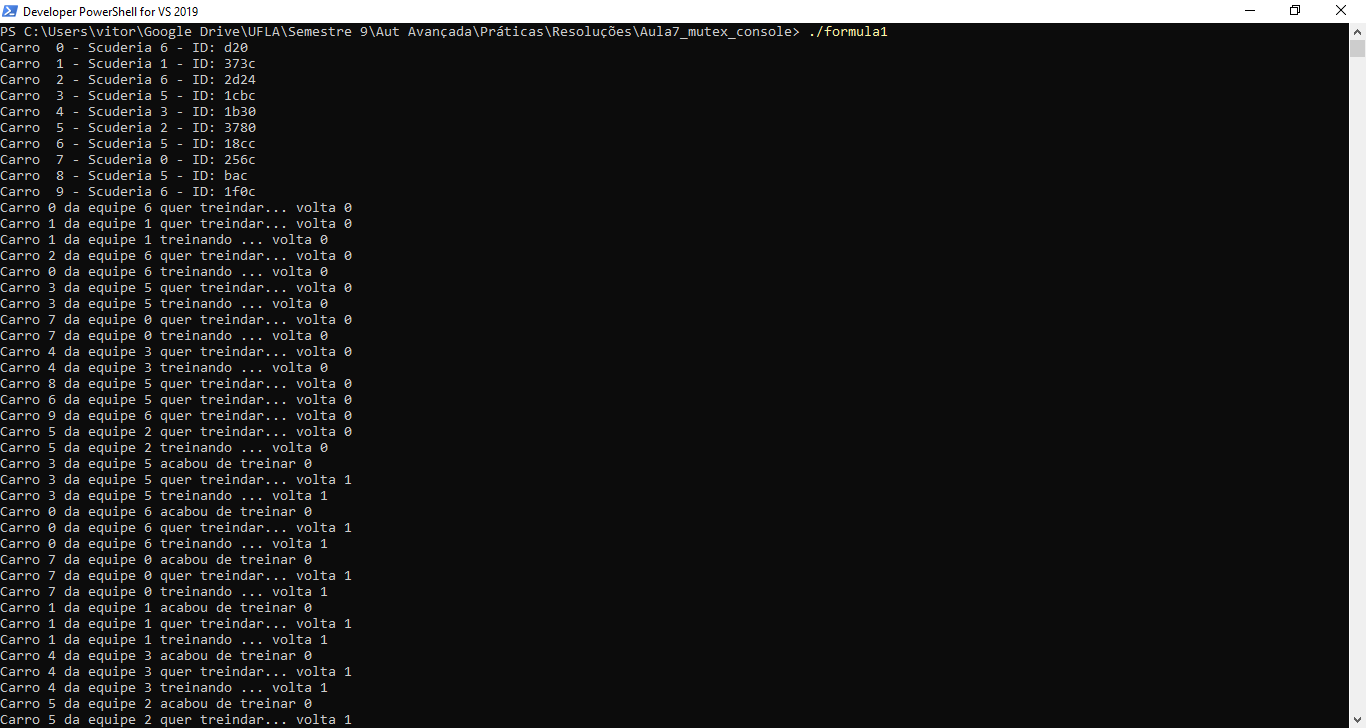
\includegraphics[width=\textwidth]{console_p1}
\caption{Teste do Programa da Tarefa 1 - Parte Superior}
\label{console_p1}
\end{figure}

\begin{figure}[H]
\centering
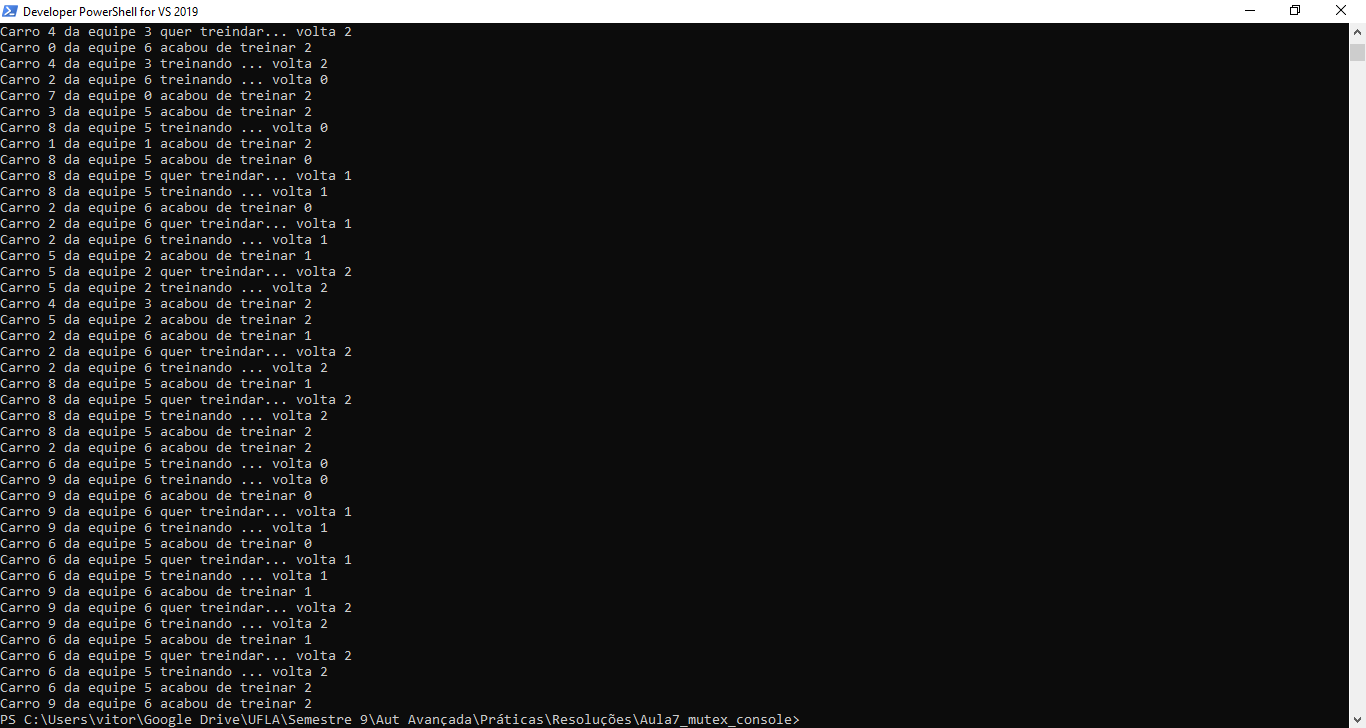
\includegraphics[width=\textwidth]{console_p2}
\caption{Teste do Programa da Tarefa 1 - Parte Superior}
\label{console_p2}
\end{figure}


\subsection*{Tarefa 2}
Aqui é apresentado o teste da aplicação com GUI. A figura \ref{qt_idle} mostra o estado inicial do programa. 

As figuras \ref{teams_10s} e \ref{teams_5s} mostram testes com tempos de descanso de 10s e 5s por volta, respectivamente. 

Pode-se notar, especialmente na figura \ref{teams_10s} que nunca há mais de 5 veículos treinando.


A figura \ref{qt_finish} mostra o comportamento do botão "Finalizar Todos os Treinos".
\begin{figure}[H]
\centering
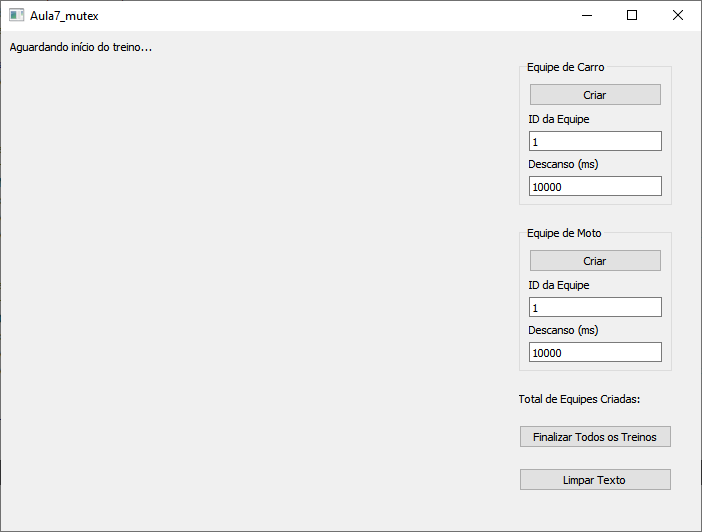
\includegraphics[width=\textwidth]{qt_idle}
\caption{Janela inicial do Programa da Tarefa 2}
\label{qt_idle}
\end{figure}

\begin{figure}[H]
\centering
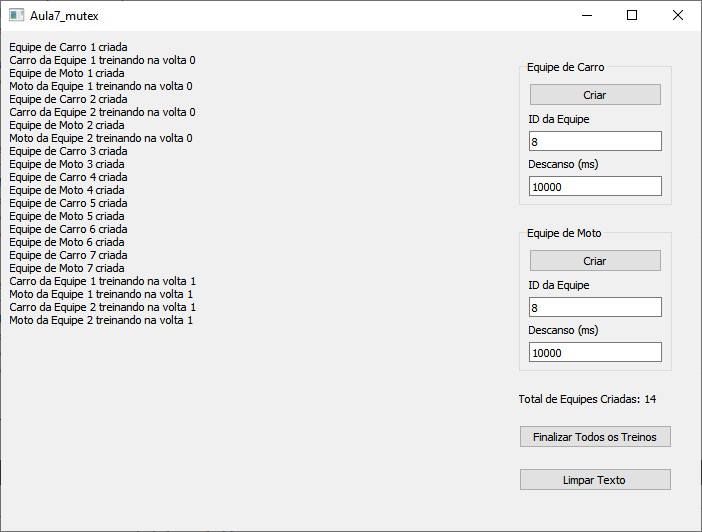
\includegraphics[width=\textwidth]{qt_teams_10s}
\caption{Teste com 10s por volta}
\label{teams_10s}
\end{figure}

\begin{figure}[H]
\centering
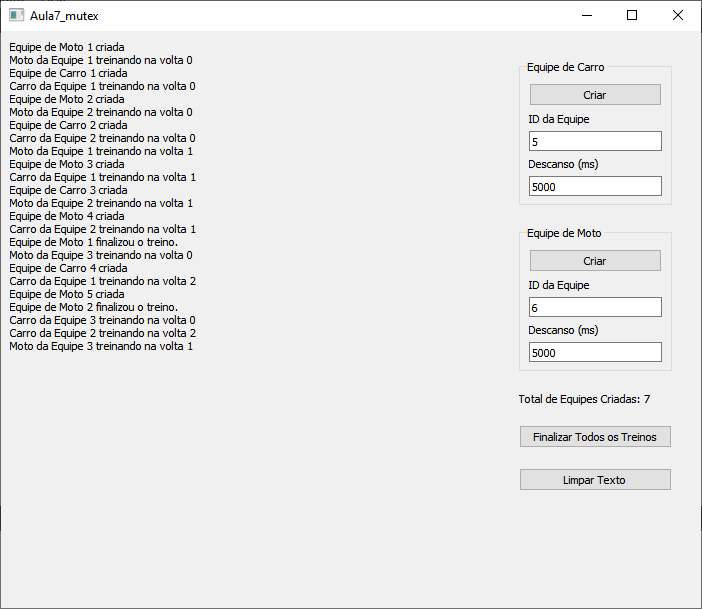
\includegraphics[width=\textwidth]{qt_teams}
\caption{Teste com 5s por volta}
\label{teams_5s}
\end{figure}

\begin{figure}[H]
\centering
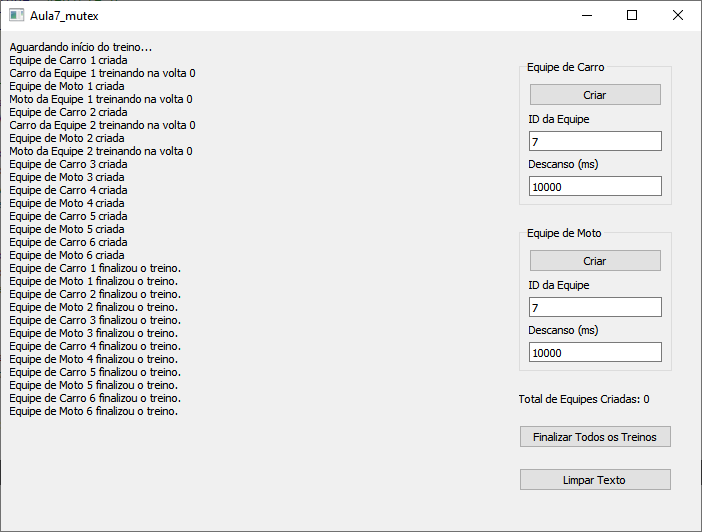
\includegraphics[width=\textwidth]{qt_finish}
\caption{Finalização Forçada dos Treinos}
\label{qt_finish}
\end{figure}

\medskip

\printbibliography

\end{document}